\chapter{Expérimentations}
\section{Donnés}\label{dataSet}
\paragraph{}Afin de tester notre solveur nous avons opté pour l'utilisation de fichiers benchmark qui vont représenter des instances du problème, dorénavant, et pour être plus conforme avec la terminologie du problème, nous utiliserons le terme \textbf{INSTANCE} pour désigner ces dits fichiers.
\paragraph{}
Les instances nous sont présentées sous forme de fichiers au format \textbf{DIMACS}\footnote{Représentation convetionnelle d'une instance du problème SAT}(plus de détails dans \ref{par:dimacs}) et sont disponibles en téléchargement gratuitement et librement dans \cite{Benchmark}, et sont également le fruit du travail de nombreux chercheurs dévoués.
\subsection{Format DIMACS}\label{par:dimacs}
Un fichier en format \textbf{DIMACS} est un fichier dont l'extension est \textbf{.cnf}, et est structuré de la manière suivante : \\
\begin{itemize}
	\item Le fichier peut commencer avec des commentaires, un commentaire sur une ligne commence par le caractère \textbf{'c'}
	\item La première ligne du fichier(après les commentaires) doit être structurée de la manière suivante : \textbf{\textcolor{green}{p cnf} \textcolor{blue}{nbvar} \textcolor{red}{nbclause}}
	\begin{enumerate}
		\item \textbf{\textcolor{green}{p cnf}} pour indiquer que l'instance est en forme normale conjonctive \textbf{FNC}.
		\item \textbf{\textcolor{blue}{nbvar}} indique le nombre de litéraux au total dans l'instance, à noté que chaque literal $x_{i}$ sera représenté par son indice $i$.
		\item \textbf{\textcolor{red}{nbclause}} le nombre total de clauses présentes dans l'instance.
	\end{enumerate}
	\item chaque ligne représente une conjonction de litéraux $(x_{i} \vert \lnot x_{i})$ indentifiés par un numero $i$, séparés par un blanc, avec un 0 à la fin pour marquer la fin de la ligne.
\end{itemize}
\subsection{Example}
c\\
c Un commentaire\\
c\\
c \\
p cnf 5 3\\
1 -5 4 0\\
-1 5 3 4 0\\
-3 -4 0\\
\subsection{Type d'instances}
Dans \cite{Benchmark} nous avons à notre disposition deux types d'instances pour chaque taille du problème : \\
\begin{itemize}
	\item Un ensemble d'instances satisfiable dans un fichier dénommé UF\textbf{\textcolor{blue}{XX}}-\textbf{\textcolor{red}{YY}}
	\item Un ensemble d'instances satisfiable dans un fichier dénommé UUF\textbf{\textcolor{blue}{XX}}-\textbf{\textcolor{red}{YY}}
	\item avec : 
	\begin{enumerate}
		\item \textbf{\textcolor{blue}{XX}} = nombre de litéraux
		\item \textbf{\textcolor{red}{YY}} = nombre de clauses
	\end{enumerate}
\end{itemize}
\newpage
\section{Environement de travail}
\subsection{Machines}\label{machines}
\paragraph{}
Pour les tests nous avons utilisé deux machines pour chaque groupes d'instances, autrement dit une machine pour effectuer les tests sur un ensembles d'instances satisfiables \textbf{\textcolor{blue}{UF75-325}}\cite{Benchmark} et une autre sur les instances contradictoires(non satisfiables) \textbf{\textcolor{red}{UUF75-325}}\cite{Benchmark}, les caractéristiques de chaque machines sont données dans les figures \ref{fig:machineA} et \ref{fig:machineB} suivantes : 
\begin{figure}[H]
	\centering
	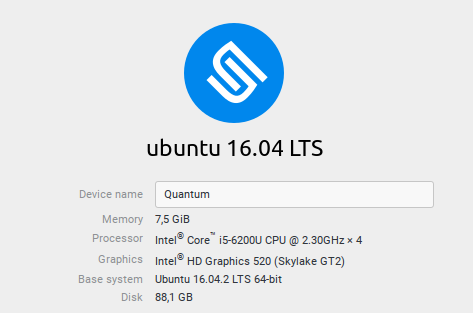
\includegraphics[scale=0.75]{images/machineWISS.png}
	\caption{Machine \textbf{A} pour les instances contradictoires}
	\label{fig:machineA}
\end{figure}
\begin{figure}[H]
	\centering
	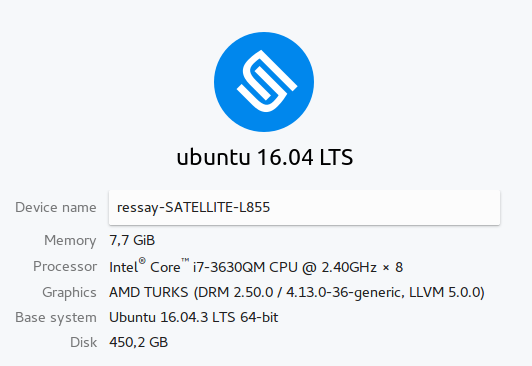
\includegraphics[scale=0.665]{images/machineYASSER.png}
	\caption{Machine \textbf{B} pour les instances satisfiables}
	\label{fig:machineB}
\end{figure}
\newpage
\subsection{Outils utilisés}
\subsubsection{Langage de programmation : }
\paragraph{}
Nous avons opté pour le langage \href{https://fr.wikipedia.org/wiki/Java_(technique)}{Java}, car il offre une grande flexibilité et un facilite l'implémentation qui est due au fait qu'il soit totallement orienté-objet.
\subsubsection{IDE : }
\paragraph{IntelliJ Idea} L'environement de dévelopement choisit est \href{https://www.jetbrains.com/idea/}{IntelliJ IDEA}, spécialement dédié au développement en utilisant le langage \href{https://fr.wikipedia.org/wiki/Java_(technique)}{Java}, il est proposé par l'entreprise \href{https://www.jetbrains.com}{JetBrains} et est caractérisé par sa forte simplicité d'utilisation et les nombreux plugins et extentions qui lui sont dédiées.

\section{Résultats}\label{tests}
\paragraph{}
Pour chacun des groupes d'instancs(i.e UF75-325 et UUF75-325) nous avons lancé les machines dédiées sur les 10 premières instances, avec 10 exécutions de durées égales à 10 mins pour chaque instance et pour chaque méthodes, les résultats sont les suivants : \\
\subsection{En largeur d'abord :}
\paragraph{}
Les résultats sont présentés d'abord sous forme de tables puis illustrés dans des histogrammes :
\paragraph{Remarque :} \label{BreadthIssueExperience} En ce qui concerne cet algorithme, nous avons eu une saturation de la mémoire après 1 min d'exécution avec la structure d'évaluation en \textbf{Bitset} (voir \ref*{def:Bitset} page \pageref{def:Bitset}) cela est principalement dû au fait que cette structure permet d'évaluer un plus grand nombre de clauses en un lapse de temps  très court là où la structure d'évaluation matrcielle ( voir \ref{def:matrix} page \pageref{def:matrix}) prend plus de temps pour faire le traitement, en conséquence le débordement de la mémoire survient mais après un temps plus conséquant, les résultats obtenus sont donc ceux observé avant le débordement.
\subsubsection{Pour les instances satisfiables :}
% Please add the following required packages to your document preamble:
% \usepackage{multirow}
\begin{table}[H]
	\centering
	\label{table:Tab_BFS_Sat}
	\begin{tabular}{|c|c|c|c|}
		\hline
		Fichiers test              & Instance & Maximum clauses & Taux  moyen de satisfiabilité \\ \hline
		\multirow{10}{*}{UF75-325} & 1        & 153             & 42,83\%                       \\ \cline{2-4} 
		& 2        & 152             & 43,94\%                       \\ \cline{2-4} 
		& 3        & 147             & 42,31\%                       \\ \cline{2-4} 
		& 4        & 140             & 42,25\%                       \\ \cline{2-4} 
		& 5        & 146             & 42,46\%                       \\ \cline{2-4} 
		& 6        & 146             & 43,05\%                       \\ \cline{2-4} 
		& 7        & 144             & 41,91\%                       \\ \cline{2-4} 
		& 8        & 160             & 44,37\%                       \\ \cline{2-4} 
		& 9        & 152             & 43,04\%                       \\ \cline{2-4} 
		& 10       & 144             & 42,58\%                       \\ \hline
	\end{tabular}
	\caption{Tableau récapitulatif des résultats pour les instances satisfiables}
\end{table}
\paragraph{}Pour mieux visualiser les données du tableau, le graphe suivant est proposé :\\

\begin{figure}[H]
	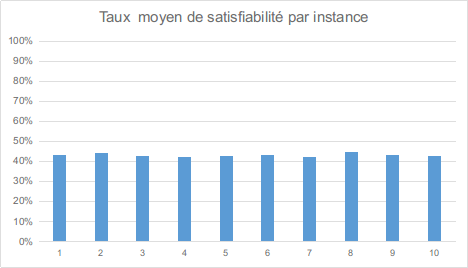
\includegraphics[width=\textwidth]{images/BFSUF75Graph.png}
	\caption{Illustration des données de \ref{table:Tab_BFS_Sat}}
\end{figure}
\newpage
\subsubsection{Pour les instances contradictoires ( non sastisfiables ) : }
% Please add the following required packages to your document preamble:
% \usepackage{multirow}
\begin{table}[H]
	\centering
	\label{table:Tab_BFS_Non_Sat}
	\begin{tabular}{|c|c|c|c|}
		\hline
		Fichiers test               & Instance & Maximum clauses & Taux moyen de satisfiabilité \\ \hline
		\multirow{10}{*}{UUF75-325} & 1        & 143             & 41,60\%                      \\ \cline{2-4} 
		& 2        & 147             & 42,95\%                      \\ \cline{2-4} 
		& 3        & 151             & 41,23\%                      \\ \cline{2-4} 
		& 4        & 136             & 41,48\%                      \\ \cline{2-4} 
		& 5        & 148             & 41,72\%                      \\ \cline{2-4} 
		& 6        & 144             & 41,05\%                      \\ \cline{2-4} 
		& 7        & 145             & 42,15\%                      \\ \cline{2-4} 
		& 8        & 145             & 41,82\%                      \\ \cline{2-4} 
		& 9        & 154             & 42,37\%                      \\ \cline{2-4} 
		& 10       & 142             & 42,15\%                      \\ \hline
	\end{tabular}
	\caption{Tableau récapitulatif des résultats pour les instances non-satisfiables}
\end{table}
\begin{figure}[H]
	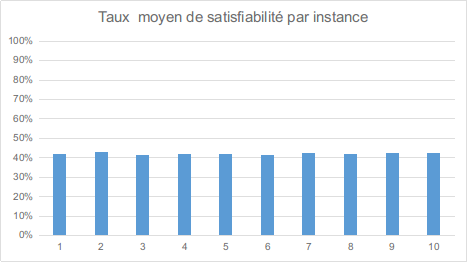
\includegraphics[width=\textwidth]{images/BFSUUF75Graph.png}
	\caption{Illustration des données de \ref{table:Tab_BFS_Non_Sat}}
\end{figure}

\newpage
\subsection{Par profondeur d'abord :}
Les résultats sont présentés d'abord sous forme de tables puis illustrés dans des histogrammes : 
\subsubsection{Pour les instances satisfiables :}
% Please add the following required packages to your document preamble:
% \usepackage{multirow}
\begin{table}[H]
	\centering
	\begin{tabular}{|c|c|c|c|}
	\hline
	Fichiers test              & Instance & Maximum clauses & Taux moyen de satisfiabilité \\ \hline
	\multirow{10}{*}{UF75-325} & 1        & 312             & 92,95\%                      \\ \cline{2-4} 
	& 2        & 306             & 92,37\%                      \\ \cline{2-4} 
	& 3        & 309             & 92,46\%                      \\ \cline{2-4} 
	& 4        & 306             & 92,65\%                      \\ \cline{2-4} 
	& 5        & 308             & 93,14\%                      \\ \cline{2-4} 
	& 6        & 310             & 94,18\%                      \\ \cline{2-4} 
	& 7        & 305             & 93,75\%                      \\ \cline{2-4} 
	& 8        & 308             & 92,49\%                      \\ \cline{2-4} 
	& 9        & 310             & 94,46\%                      \\ \cline{2-4} 
	& 10       & 306             & 94,22\%                      \\ \hline
\end{tabular}
	\caption{Tableau récapitulatif des résultats pour les instances satisfiables}
	\label{table:Tab_DFS_Sat}
\end{table}
\begin{figure}[H]
	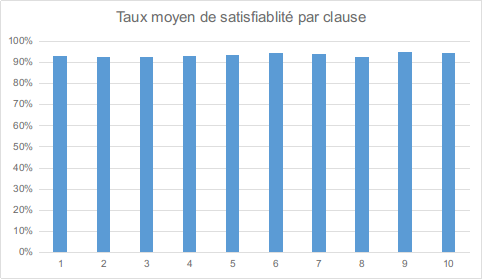
\includegraphics[width=\textwidth]{images/DFSUF75Graph.png}
	\caption{Illustration des données de la table \ref{table:Tab_DFS_Sat}}
\end{figure}


\subsubsection{Pour les instances contradictoires ( non sastisfiables ) :  }
% Please add the following required packages to your document preamble:
% \usepackage{multirow}
\begin{table}[H]
	\centering
	\begin{tabular}{|c|c|c|c|}
		\hline
		Fichiers test              & Instance & Maximum clauses & Taux moyen de satisfiabilité \\ \hline
		\multirow{10}{*}{UF75-325} & 1        & 312             & 94,37\%                      \\ \cline{2-4} 
		& 2        & 306             & 93,29\%                      \\ \cline{2-4} 
		& 3        & 309             & 94,34\%                      \\ \cline{2-4} 
		& 4        & 306             & 92,83\%                      \\ \cline{2-4} 
		& 5        & 308             & 92,61\%                      \\ \cline{2-4} 
		& 6        & 310             & 95,38\%                      \\ \cline{2-4} 
		& 7        & 305             & 92,83\%                      \\ \cline{2-4} 
		& 8        & 308             & 93,66\%                      \\ \cline{2-4} 
		& 9        & 310             & 93,60\%                      \\ \cline{2-4} 
		& 10       & 306             & 93,33\%                      \\ \hline
	\end{tabular}
	\caption{Tableau récapitulatif des résultats pour les instances non-satisfiables}
	\label{table:Tab_DFS_Non_Sat}
\end{table}
\begin{figure}[H]
	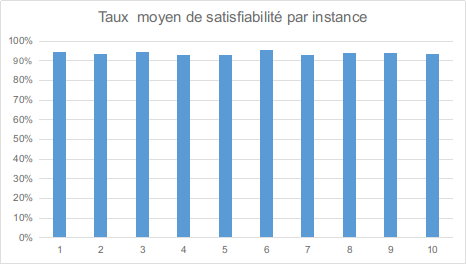
\includegraphics[width=\textwidth]{images/DFSUUF75Graph.png}
	\caption{Illustration des données de la table \ref{table:Tab_DFS_Non_Sat}}
\end{figure}
%%%%%%%%%%%%%%%%%%%%%%%%%%%%%%%%%%%%%%%%%%%%%%%%%%%%%%%%%%%%%%%%
\newpage
\subsection{Cout uniforme} :
Les résultats sont présentés d'abord sous forme de tables puis illustrés dans des histogrammes : 
\subsubsection{Pour les instances satisfiables :}
% Please add the following required packages to your document preamble:
% \usepackage{multirow}
\begin{table}[H]
	\centering
	\begin{tabular}{|c|c|c|c|}
		\hline
		Fichiers test               & Instance & Maximum clauses & Taux moyen de satisfiabilité \\ \hline
		\multirow{10}{*}{UF75-325} & 1        & 307             & 93,38\%                      \\ \cline{2-4} 
		& 2        & 304             & 93,23\%                      \\ \cline{2-4} 
		& 3        & 307             & 93,23\%                      \\ \cline{2-4} 
		& 4        & 304             & 92,77\%                      \\ \cline{2-4} 
		& 5        & 303             & 93,08\%                      \\ \cline{2-4} 
		& 6        & 302             & 92,77\%                      \\ \cline{2-4} 
		& 7        & 299             & 91,69\%                      \\ \cline{2-4} 
		& 8        & 301             & 92,00\%                      \\ \cline{2-4} 
		& 9        & 307             & 93,54\%                      \\ \cline{2-4} 
		& 10       & 305             & 93,08\%                      \\ \hline
	\end{tabular}
	\caption{Tableau récapitulatif des résultats pour les instances satisfiables}
	\label{table:Tab_UniformCost_Sat}
\end{table}
\begin{figure}[H]
	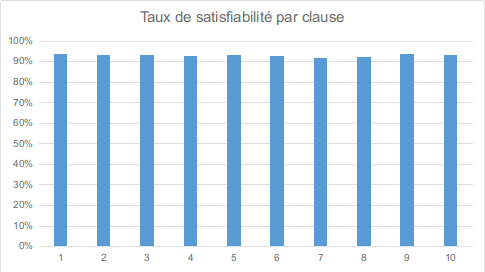
\includegraphics[width=\textwidth]{images/UniformCostUF75Graph.png}
	\caption{Illustration des données de la table \ref{table:Tab_UniformCost_Sat}}
\end{figure}


\subsubsection{Pour les instances contradictoires ( non sastisfiables ) :  }
% Please add the following required packages to your document preamble:
% \usepackage{multirow}
\begin{table}[H]
	\centering
	\begin{tabular}{|c|c|c|c|}
		\hline
		Fichiers test              & Instance & Maximum clauses & Taux moyen de satisfiabilité \\ \hline
		\multirow{10}{*}{UUF75-325} & 1        & 299             & 91,69\%                      \\ \cline{2-4} 
		& 2        & 305             & 92,77\%                      \\ \cline{2-4} 
		& 3        & 301             & 92,00\%                      \\ \cline{2-4} 
		& 4        & 307             & 94,15\%                      \\ \cline{2-4} 
		& 5        & 309             & 94,92\%                      \\ \cline{2-4} 
		& 6        & 300             & 92,00\%                      \\ \cline{2-4} 
		& 7        & 303             & 92,92\%                      \\ \cline{2-4} 
		& 8        & 301             & 92,46\%                      \\ \cline{2-4} 
		& 9        & 310             & 94,62\%                      \\ \cline{2-4} 
		& 10       & 308             & 94,42\%                      \\ \hline
	\end{tabular}
	\caption{Tableau récapitulatif des résultats pour les instances non-satisfiables}
	\label{table:Tab_UniformCost_Non_Sat}
\end{table}
\begin{figure}[H]
	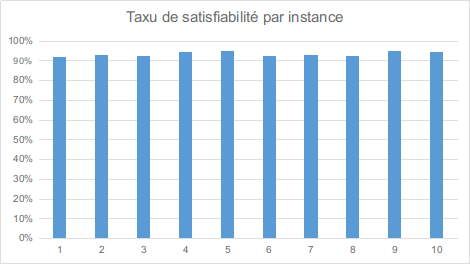
\includegraphics[width=\textwidth]{images/UniformCostUUF75Graph.png}
	\caption{Illustration des données de la table \ref{table:Tab_UniformCost_Non_Sat}}
\end{figure}

%%%%%%%%%%%%%%%%%%%%%%%%%%%%%%%%%%%%%%%%%%%%%%%%%%%%%%%%%%%%%%%%%

%%%%%%%%%%%%%%%%%%%%%%%%%%%%%%%%%%%%%%%%%%%%%%%%%%%%%%%%%%%%%%%%
\newpage
\subsection{Recherche gloutonne} :
Les résultats sont présentés d'abord sous forme de tables puis illustrés dans des histogrammes : 
\subsubsection{Pour les instances satisfiables :}
% Please add the following required packages to your document preamble:
% \usepackage{multirow}
\begin{table}[H]
	\centering
	\begin{tabular}{|c|c|c|c|}
		\hline
		Fichiers test              & Instance & Maximum clauses & Taux moyen de satisfiabilité \\ \hline
		\multirow{10}{*}{UF75-325} & 1        & 320             & 98,15\%                      \\ \cline{2-4} 
		& 2        & 319             & 97,85\%                      \\ \cline{2-4} 
		& 3        & 316             & 96,77\%                      \\ \cline{2-4} 
		& 4        & 317             & 97,23\%                      \\ \cline{2-4} 
		& 5        & 317             & 97,23\%                      \\ \cline{2-4} 
		& 6        & 317             & 97,08\%                      \\ \cline{2-4} 
		& 7        & 315             & 96,46\%                      \\ \cline{2-4} 
		& 8        & 318             & 97,23\%                      \\ \cline{2-4} 
		& 9        & 318             & 97,54\%                      \\ \cline{2-4} 
		& 10       & 316             & 97,08\%                      \\ \hline
	\end{tabular}
	\caption{Tableau récapitulatif des résultats pour les instances satisfiables}
	\label{table:Tab_Greedy_Sat}
\end{table}
\begin{figure}[H]
	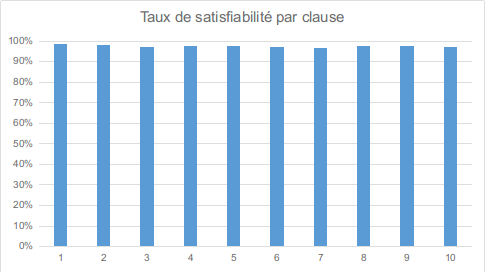
\includegraphics[width=\textwidth]{images/GreedyUF75Graph.png}
	\caption{Illustration des données de la table \ref{table:Tab_Greedy_Sat}}
\end{figure}


\subsubsection{Pour les instances contradictoires ( non sastisfiables ) :  }
% Please add the following required packages to your document preamble:
% \usepackage{multirow}
\begin{table}[H]
	\centering
	\begin{tabular}{|c|c|c|c|}
		\hline
		Fichiers test               & Instance & Maximum clauses & Taux moyen de satisfiabilité \\ \hline
		\multirow{10}{*}{UUF75-325} & 1        & 316             & 96,31\%                      \\ \cline{2-4} 
		& 2        & 315             & 96,77\%                      \\ \cline{2-4} 
		& 3        & 316             & 96,77\%                      \\ \cline{2-4} 
		& 4        & 313             & 96,31\%                      \\ \cline{2-4} 
		& 5        & 315             & 96,77\%                      \\ \cline{2-4} 
		& 6        & 311             & 95,08\%                      \\ \cline{2-4} 
		& 7        & 313             & 95,85\%                      \\ \cline{2-4} 
		& 8        & 314             & 96,00\%                      \\ \cline{2-4} 
		& 9        & 320             & 98,00\%                      \\ \cline{2-4} 
		& 10       & 310             & 94,92\%                      \\ \hline
	\end{tabular}
	\caption{Tableau récapitulatif des résultats pour les instances non-satisfiables}
	\label{table:Tab_Greedy_Non_Sat}
\end{table}
\begin{figure}[H]
	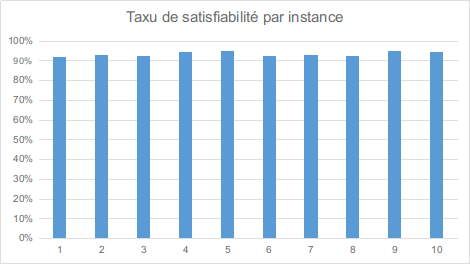
\includegraphics[width=\textwidth]{images/UniformCostUUF75Graph.png}
	\caption{Illustration des données de la table \ref{table:Tab_Greedy_Non_Sat}}
\end{figure}

%%%%%%%%%%%%%%%%%%%%%%%%%%%%%%%%%%%%%%%%%%%%%%%%%%%%%%%%%%%%%%%%%


\newpage
\subsection{Algorithme A*} :
Les résultats sont présentés d'abord sous forme de tables puis illustrés dans des histogrammes : 
\subsubsection{Pour les instances satisfiables :}
% Please add the following required packages to your document preamble:
% \usepackage{multirow}
\begin{table}[H]
	\centering
	\begin{tabular}{|c|c|c|c|}
		\hline
		Fichiers test              & Instance & Maximum clauses & Taux moyen de satisfiabilité \\ \hline
		\multirow{10}{*}{UF75-325} & 1        & 318             & 96,58\%                      \\ \cline{2-4} 
		& 2        & 318             & 97,26\%                      \\ \cline{2-4} 
		& 3        & 316             & 96,25\%                      \\ \cline{2-4} 
		& 4        & 316             & 96,31\%                      \\ \cline{2-4} 
		& 5        & 320             & 97,42\%                      \\ \cline{2-4} 
		& 6        & 320             & 97,20\%                      \\ \cline{2-4} 
		& 7        & 318             & 96,80\%                      \\ \cline{2-4} 
		& 8        & 319             & 96,83\%                      \\ \cline{2-4} 
		& 9        & 319             & 97,29\%                      \\ \cline{2-4} 
		& 10       & 319             & 97,54\%                      \\ \hline
	\end{tabular}
	\caption{Tableau récapitulatif des résultats pour les instances satisfiables}
	\label{table:Tab_Astar_Sat}
\end{table}
\begin{figure}[H]
	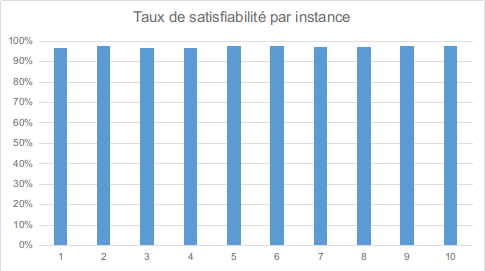
\includegraphics[width=\textwidth]{images/AstarUF75Graph.png}
	\caption{Illustration des données de la table \ref{table:Tab_Astar_Sat}}
\end{figure}


\subsubsection{Pour les instances contradictoires ( non sastisfiables ) :  }
% Please add the following required packages to your document preamble:
% \usepackage{multirow}
\begin{table}[H]
	\centering
\begin{tabular}{|c|c|c|c|}
	\hline
	Fichiers test               & Instance & Maximum clauses & Taux moyen de satisfiabilité \\ \hline
	\multirow{10}{*}{UUF75-325} & 1        & 316             & 94,65\%                      \\ \cline{2-4} 
	& 2        & 317             & 95,31\%                      \\ \cline{2-4} 
	& 3        & 315             & 94,33\%                      \\ \cline{2-4} 
	& 4        & 315             & 94,38\%                      \\ \cline{2-4} 
	& 5        & 320             & 95,47\%                      \\ \cline{2-4} 
	& 6        & 320             & 95,26\%                      \\ \cline{2-4} 
	& 7        & 317             & 94,86\%                      \\ \cline{2-4} 
	& 8        & 319             & 94,89\%                      \\ \cline{2-4} 
	& 9        & 318             & 95,34\%                      \\ \cline{2-4} 
	& 10       & 318             & 95,59\%                      \\ \hline
\end{tabular}
	\caption{Tableau récapitulatif des résultats pour les instances non-satisfiables}
	\label{table:Tab_Astar_Non_Sat}
\end{table}
\begin{figure}[H]
	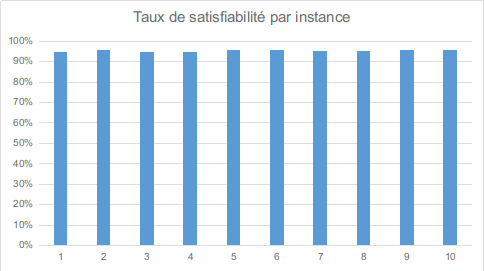
\includegraphics[width=\textwidth]{images/AstarUUF75Graph.png}
	\caption{Illustration des données de la table \ref{table:Tab_Astar_Non_Sat}}
\end{figure}
\newpage
\section{Statistiques}
\paragraph{}
Étant donné le très grand nombre de données et de résultats obtenus, nous avons décidé de récapitulé ces dérniers dans un tableau statistiques, puis dans un graphique de type \textbf{Boites-à-moustaches}

%-------------------------------------------------------------------------------
\begin{table}[H]
	\centering
	\resizebox{\textwidth}{!}{%
		\begin{tabular}{|c|c|c|c|c|c|}
			\hline
			\multicolumn{6}{|c|}{\multirow{2}{*}{UF75-325}}                                                               \\
			\multicolumn{6}{|c|}{}                                                                                        \\ \hline
			Mesure                              & BFS       & DFS       & Coût Uniforme & Recherche Gloutonne & A*        \\ \hline
			Nombre moyen de clauses satisfaites & 139,4     & 303,1     & 303,0         & 314,0               & 316,1     \\ \hline
			Taux Moyen de satisfiablié          & 42,9021\% & 93,2677\% & 93,2154\%     & 96,6000\%           &  97,2615\% \\ \hline
		\end{tabular}%
	}
	\caption{Tableau de mesures statistiques pour les instances satifsiables}
	\label{table:stat_sat}
\end{table}
\begin{figure}[H]
	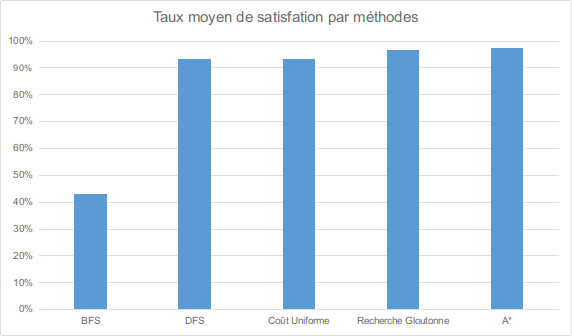
\includegraphics[width=\textwidth]{images/CompareUF75.png}
	\caption{Illustration des données de la table \ref{table:stat_sat}}
\end{figure}
\newpage
%------------------------------------------------------------------------------
\begin{table}[H]
	\centering
	
	\resizebox{\textwidth}{!}{%
		\begin{tabular}{|c|c|c|c|c|c|}
			\hline
			\multicolumn{6}{|c|}{\multirow{2}{*}{UUF75-325}}                                                               \\
			\multicolumn{6}{|c|}{}                                                                                        \\ \hline
			Mesure                              & BFS       & DFS       & Coût uniforme & Recherche gloutonne & A*        \\ \hline
			Nombre moyen de clauses satisfaites & 136,0     & 304,3     & 301,9         & 312,9               & 315,1     \\ \hline
			Taux Moyen de satisfiablié          & 41,8523\% & 93,6246\% & 92,8769\%     & 96,2769\%           & 96,9477\% \\ \hline
		\end{tabular}%
	}
	\caption{Tableau de mesures statistiques pour les instances non-satifsiables}
	\label{table:stat_non_sat}
\end{table}
%------------------------------------------------------------------------------

\begin{figure}[H]
	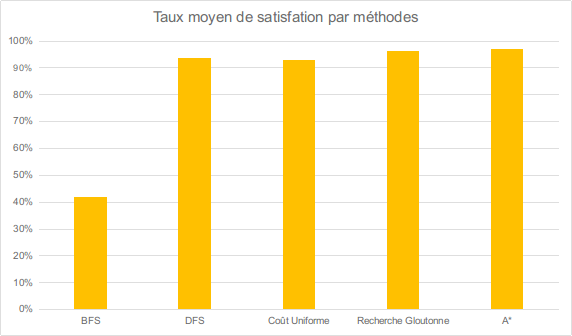
\includegraphics[width=\textwidth]{images/CompareUUF75.png}
	\caption{Illustration des données de la table \ref{table:stat_non_sat}}
\end{figure}
%------------------------------------------------------------------------------

\subsubsection{Améliorations avec BitSet}
\paragraph{}
Nous avons tenté de comparé les résultats expérimentaux en essayant différentes structures de données pour l'évaluation d'une solution et la gestion de la liste open, le tableau suivant ( voir table \ref{tab:bitsetIsLayfu} )  \ démontre que la structure du BitSet proposée évalue 15 à 190 fois ( selon la géstion de open ) plus de clauses en une seconde que la struture de matrice, combiner cette représentation avec une gesion en tas de open, nous a fait gagné un temps assez important lors de l'évaluation et le réarrangement de open.
\begin{center}\label{tab:bitsetIsLayfu}
	\begin{tabular}{|c | c| c|}
		\hline
		\backslashbox{gestion de open}{évaluation par}& Matrice & Bitset\\\hline
		liste triée& 205124 éval/s& 11952330 éval/s\\\hline
		tas & 237532 éval/s & 37252319 éval/s\\\hline
		FIFO & 238403 éval/s & 3149722 éval/s\\\hline
		LIFO & 213397 éval/s& 40879427 éval/s\\\hline
		\end{tabular}
		\captionof{table}{Nombre d'évaluations par seconde} 
\end{center}
		
		
		
\section{Comparaison entres les cinq méthodes}
\paragraph{}
Pour conclure ce chapitre, nous allons mainetant comparer les différentes méthodes selon la rapidité d'exécution, l'espace mémoire utilisé et le taux de satisfiabilité enregistré.
\paragraph{}
Nous avons remarqué à travers les nombreux tests que les deux catégories de stratégies de recherche avaient des forces et des lacunes, pour citer des exemples, la recherche par profondeur d'abord et en largeur d'abord de part sa simplicité, sont de bonnes stratégies de recherche, mais dont les limites sont vites atteintes, la première est certe peu gourmande en espace mémoire, mais ne trouve pas la solution en un temps assez rapide, la deuxième quant à elle nous garantie (si le coût pour passer d'un noeud à un autre est le même quelques soient les noeuds choisis) de trouver la solution avec le plus petit nombre de litéraux possible, mais en contre partie consomme énormemment de mémoire, ce qui peut conduire à un débordement de la mémoire très rapidement\label{BreadthIssueCompare}.
\paragraph{}
Pour ce qu'il en est de l'agrotithme de recherche par coût uniforme, il se voit être un compromis entre l'agorithme DFS\footnote{Depth first search} (voir \ref{DFSdef}) et l'algorithme BFS(\footnote{Breadth first search} (voir \ref{BFSdef}, il assure de trouver la solution avec un potentiel débordement de mémoire, mais peut aussi prendre un temps exponentiel pour trouver la solution (\ref{DijkstraDef}), les expérimentations réalisés en sont la preuve.
\paragraph{}
Quand on bascule vers la deuxième catégorie, on se rend vite commpte que l'ajout d'une heuristique peut réduire le temps de recherche d'une façon significative, ce que fait l'algorithme DFS en 10-15 mins peut être fait en quelques secondes avec l'algorithme de recherches gloutonne ou bien A*, cependant le gain en rapidité ne masque pas le fait que l'espace mémoire reste aussi soumis à un débordement ( moins fréquemment mais ça reste un risque potentiel), de plus la difficulté de trouver de bonnes heuristiques ( admissibles par exemple ) demeure un challenge du point de vue théorique et pratique, à noté aussi que très souvent, l'algorithme A* se limite à une recherche dans un maximum local, ce qui peut ralentir le processus de recherche de solutions optimales.
\paragraph{}
Une remarque à faire concernant l'ensemble des méthodes utilisées est que les résultats, malgré le fait que le choix des noeuds soit àléatoire, ne diffèrent pas d'une exécution à une autre sur une même instance ( pour A* par exemple on est dans les 96\%-97\% de taux de satisfiabilité sur les benchmarks fournis) , cela est dû principalement au fait que les fréquences d'apparitions des litéraux soient très proches les unes des autres, aisni choisir un litéral (ou sa négation) plutôt qu'un autre n'influe pas vraiment sur le résultat final.